% Get the selected campground data from the brewing function


\documentclass{article}\usepackage[]{graphicx}\usepackage[]{color}
%% maxwidth is the original width if it is less than linewidth
%% otherwise use linewidth (to make sure the graphics do not exceed the margin)
\makeatletter
\def\maxwidth{ %
  \ifdim\Gin@nat@width>\linewidth
    \linewidth
  \else
    \Gin@nat@width
  \fi
}
\makeatother

\definecolor{fgcolor}{rgb}{0.345, 0.345, 0.345}
\newcommand{\hlnum}[1]{\textcolor[rgb]{0.686,0.059,0.569}{#1}}%
\newcommand{\hlstr}[1]{\textcolor[rgb]{0.192,0.494,0.8}{#1}}%
\newcommand{\hlcom}[1]{\textcolor[rgb]{0.678,0.584,0.686}{\textit{#1}}}%
\newcommand{\hlopt}[1]{\textcolor[rgb]{0,0,0}{#1}}%
\newcommand{\hlstd}[1]{\textcolor[rgb]{0.345,0.345,0.345}{#1}}%
\newcommand{\hlkwa}[1]{\textcolor[rgb]{0.161,0.373,0.58}{\textbf{#1}}}%
\newcommand{\hlkwb}[1]{\textcolor[rgb]{0.69,0.353,0.396}{#1}}%
\newcommand{\hlkwc}[1]{\textcolor[rgb]{0.333,0.667,0.333}{#1}}%
\newcommand{\hlkwd}[1]{\textcolor[rgb]{0.737,0.353,0.396}{\textbf{#1}}}%
\let\hlipl\hlkwb

\usepackage{framed}
\makeatletter
\newenvironment{kframe}{%
 \def\at@end@of@kframe{}%
 \ifinner\ifhmode%
  \def\at@end@of@kframe{\end{minipage}}%
  \begin{minipage}{\columnwidth}%
 \fi\fi%
 \def\FrameCommand##1{\hskip\@totalleftmargin \hskip-\fboxsep
 \colorbox{shadecolor}{##1}\hskip-\fboxsep
     % There is no \\@totalrightmargin, so:
     \hskip-\linewidth \hskip-\@totalleftmargin \hskip\columnwidth}%
 \MakeFramed {\advance\hsize-\width
   \@totalleftmargin\z@ \linewidth\hsize
   \@setminipage}}%
 {\par\unskip\endMakeFramed%
 \at@end@of@kframe}
\makeatother

\definecolor{shadecolor}{rgb}{.97, .97, .97}
\definecolor{messagecolor}{rgb}{0, 0, 0}
\definecolor{warningcolor}{rgb}{1, 0, 1}
\definecolor{errorcolor}{rgb}{1, 0, 0}
\newenvironment{knitrout}{}{} % an empty environment to be redefined in TeX

\usepackage{alltt}

\title{Analysis of Cereal data K}

\author{Carl James Schwarz}

%\date{}
\IfFileExists{upquote.sty}{\usepackage{upquote}}{}
\begin{document}

\maketitle




\section{Introduction}
What is the relationship between the calories in a serving of breakfast
cereal and the placement of the cereal on the shelf in the supermarket?


\section{Material and Methods}
A sample of 23 cereals were sampled from a local grocery store
and the nutritional information (e.g. number of grams of fat, protein, carbohydrates, etc.)
and the number of calories per serving was extracted. 
The display shelf on which the cereal was stored was also recorded.

Regression analysis was used to look at the relationship between
the calories per serving and the fat content per serving.

All computations were performed using R version 3.5.2 (2018-12-20).


\section{Results}
The data was screened for outliers and no unusal points were located.

Table~\ref{tab:table1} summarizes the calories per serving by shelf number.
%latex.default(report, file = "", where = "b", rowname = NULL,     caption = "Summary statistics by shelf location", label = "tab:table1",     colheads = colheads, col.just = c("l", rep("r", 5)))%
\begin{table}[b]
\caption{Summary statistics by shelf location\label{tab:table1}} 
\begin{center}
\begin{tabular}{lrrrrr}
\hline\hline
\multicolumn{1}{c}{Shelf}&\multicolumn{1}{c}{n}&\multicolumn{1}{c}{Mean}&\multicolumn{1}{c}{Min}&\multicolumn{1}{c}{Max}&\multicolumn{1}{c}{SD}\tabularnewline
&&\multicolumn{1}{c}{{\scriptsize calories}}&\multicolumn{1}{c}{{\scriptsize calories}}&\multicolumn{1}{c}{{\scriptsize calories}}&\multicolumn{1}{c}{{\scriptsize calories}}\tabularnewline
\hline
Low&$ 4$&$105.0$&$100$&$110$&$ 5.8$\tabularnewline
Middle&$ 7$&$107.1$&$ 90$&$120$&$11.1$\tabularnewline
High&$12$&$106.7$&$ 50$&$160$&$30.8$\tabularnewline
\hline
\end{tabular}\end{center}
\end{table}


Figure~\ref{fig:scatter} shows a graphical display of the calories per serving.



\begin{figure}[h] 
\begin{center} 
\begin{knitrout}
\definecolor{shadecolor}{rgb}{0.969, 0.969, 0.969}\color{fgcolor}
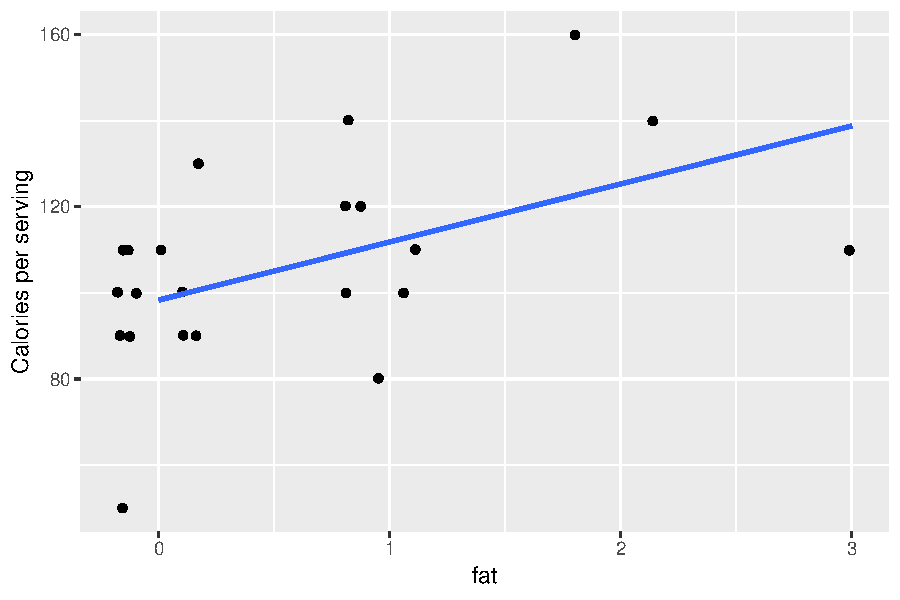
\includegraphics[width=\maxwidth]{figure/unnamed-chunk-1-1} 

\end{knitrout}
\end{center}
\caption{Calories by shelf height}
\label{fig:scatter}
\end{figure}




There was no evidence  of a difference in the mean calories per serving
varied with the amount of fat (p=0.989).
The estimated slope was 
1.18 (SE
9.71).

\section{Summary}
We found no
evidence that the mean number of calories varied with fat content.


\end{document}
# we need a blank line at the end (See Reproducible Research with R and Rstudio, page 247)

